\documentclass[aspectratio=169,10pt]{beamer}

\usepackage[utf8]{inputenc}
\usepackage[T1]{fontenc}
\usepackage[french]{babel}
\AtBeginDocument{\shorthandoff{;:!?}}
\usepackage{amssymb}
\usepackage{lmodern}
\usepackage{graphicx}
\usepackage{tikz}
\usetikzlibrary{shapes.geometric,arrows.meta,positioning,calc,fit,backgrounds,shapes.multipart,decorations.pathreplacing}
\usetikzlibrary{babel}
\usepackage{listings}
\usepackage{xcolor}
\usepackage{booktabs}
\usepackage{array}
\usepackage{colortbl}
\usepackage{hyperref}

\definecolor{myblue}{RGB}{27,63,139}
\definecolor{mybluelight}{RGB}{74,134,200}
\definecolor{mybluepale}{RGB}{232,240,251}
\definecolor{myaccent}{RGB}{230,100,20}
\definecolor{mysuccess}{RGB}{34,139,68}
\definecolor{codebg}{RGB}{245,247,250}
\definecolor{mygray}{RGB}{100,100,100}

\usetheme{Boadilla}
\usecolortheme[named=myblue]{structure}

\setbeamercolor{palette primary}{bg=myblue,fg=white}
\setbeamercolor{palette secondary}{bg=mybluelight,fg=white}
\setbeamercolor{palette tertiary}{bg=myblue!80,fg=white}
\setbeamercolor{palette quaternary}{bg=myblue,fg=white}
\setbeamercolor{frametitle}{bg=myblue,fg=white}
\setbeamercolor{title}{fg=white}
\setbeamercolor{subtitle}{fg=white!80}
\setbeamercolor{block title}{bg=myblue!90,fg=white}
\setbeamercolor{block body}{bg=mybluepale!60}
\setbeamercolor{alerted text}{fg=myaccent}
\setbeamercolor{block title alerted}{bg=myaccent,fg=white}
\setbeamercolor{block body alerted}{bg=myaccent!10}
\setbeamercolor{block title example}{bg=mysuccess!80,fg=white}
\setbeamercolor{block body example}{bg=mysuccess!12}
\setbeamercolor{itemize item}{fg=myblue}
\setbeamercolor{itemize subitem}{fg=mybluelight}
\setbeamercolor{enumerate item}{fg=myblue}

\setbeamertemplate{navigation symbols}{}
\setbeamertemplate{itemize item}{\color{myblue}\small$\blacktriangleright$}
\setbeamertemplate{itemize subitem}{\color{mybluelight}\small$\triangleright$}
\setbeamertemplate{enumerate item}{\color{myblue}\textbf{\insertenumlabel.}}

\setbeamerfont{frametitle}{series=\bfseries,size=\normalsize}
\setbeamerfont{block title}{series=\bfseries,size=\small}
\setbeamerfont{block body}{size=\small}

\AtBeginSection[]{
  \begin{frame}[plain]
    \begin{tikzpicture}[remember picture,overlay]
      \fill[myblue] (current page.north west) rectangle (current page.south east);
      \fill[mybluelight!40,opacity=0.5]
        (current page.south west) rectangle ++(\paperwidth,1.4cm);
    \end{tikzpicture}
    \vfill
    \begin{center}
    {\color{white!60}\large\textit{Partie \thesection}}\\[8pt]
    {\color{white}\LARGE\bfseries\insertsectionhead}
    \end{center}
    \vfill
  \end{frame}
}

\lstdefinestyle{pysmall}{
    language=Python,
    basicstyle=\ttfamily\tiny,
    keywordstyle=\color{myblue}\bfseries,
    commentstyle=\color{mygray}\itshape,
    stringstyle=\color{myaccent},
    showstringspaces=false,
    breaklines=true,
    frame=single,
    rulecolor=\color{myblue!30},
    backgroundcolor=\color{codebg},
    numbers=left,
    numberstyle=\tiny\color{mygray},
    numbersep=4pt,
    tabsize=4,
    xleftmargin=6pt,
    framexleftmargin=6pt,
}
\lstdefinestyle{sqlsmall}{
    language=SQL,
    basicstyle=\ttfamily\tiny,
    keywordstyle=\color{myblue}\bfseries,
    commentstyle=\color{mygray}\itshape,
    stringstyle=\color{myaccent},
    showstringspaces=false,
    breaklines=true,
    frame=single,
    rulecolor=\color{myblue!30},
    backgroundcolor=\color{codebg},
    tabsize=2,
    xleftmargin=6pt,
}

\tikzset{
  syst/.style={rectangle,draw=myblue,thick,rounded corners=4pt,fill=mybluepale,
    align=center,minimum height=10mm,minimum width=28mm,font=\bfseries\scriptsize},
  box/.style={rectangle,draw=myblue,rounded corners=3pt,fill=mybluepale,
    align=center,minimum height=7mm,inner sep=5pt,font=\scriptsize},
  extbox/.style={rectangle,draw=mygray,fill=gray!10,align=center,
    minimum height=8mm,inner sep=5pt,font=\scriptsize},
  comp/.style={rectangle,draw=myblue,fill=mybluepale,align=center,
    minimum height=10mm,minimum width=30mm,inner sep=5pt,font=\scriptsize},
  layer/.style={rectangle,draw=myblue,rounded corners=3pt,align=center,
    minimum height=10mm,minimum width=42mm,inner sep=5pt,font=\scriptsize},
  flow/.style={-{Stealth[length=2mm]},thick,color=myblue},
  flowlab/.style={font=\tiny,fill=white,inner sep=1pt},
  dep/.style={-{Stealth[length=2mm]},thick,dashed,color=mybluelight},
  act/.style={rectangle,rounded corners=3pt,draw=myblue,fill=mybluepale,
    align=center,minimum height=6mm,minimum width=26mm,font=\scriptsize,inner sep=3pt},
  decision/.style={diamond,draw=myblue,fill=orange!15,aspect=2.2,
    align=center,font=\tiny,inner sep=0pt},
  init/.style={circle,draw=myblue,fill=myblue,minimum size=4mm,inner sep=0pt},
  final/.style={circle,draw=myblue,minimum size=5.5mm,inner sep=0pt,
    path picture={\fill[myblue] (path picture bounding box.center) circle (1.5mm);}},
  tag/.style={rectangle,rounded corners=2pt,fill=myblue,text=white,
    font=\tiny\bfseries,inner sep=2.5pt},
  taggreen/.style={rectangle,rounded corners=2pt,fill=mysuccess,text=white,
    font=\tiny\bfseries,inner sep=2.5pt},
  tagorange/.style={rectangle,rounded corners=2pt,fill=myaccent,text=white,
    font=\tiny\bfseries,inner sep=2.5pt},
  tbl/.style={rectangle,draw=myblue,fill=white,font=\scriptsize,
    rectangle split,rectangle split parts=2,align=left,inner sep=3pt,text width=26mm},
  usecase/.style={ellipse,draw=myblue,fill=mybluepale,align=center,
    minimum width=26mm,minimum height=8mm,font=\tiny,inner sep=1pt},
  ucsys/.style={rectangle,draw=myblue,thick,rounded corners=2pt},
  actorbox/.style={rectangle,draw=myblue,fill=mybluepale,font=\tiny\bfseries,
    minimum height=6mm,align=center,inner sep=3pt},
  lifeline/.style={dashed,color=mygray!70},
  seqmsg/.style={-{Stealth[length=1.6mm]},font=\tiny,color=myblue},
  seqret/.style={-{Stealth[length=1.6mm]},dashed,font=\tiny,color=mygray},
}

\newcommand{\umlactor}[3]{
  \begin{scope}[shift={(#1,#2)}]
    \draw[thick,myblue] (0,0.55) circle (0.14);
    \draw[thick,myblue] (0,0.41) -- (0,-0.05);
    \draw[thick,myblue] (-0.22,0.26) -- (0.22,0.26);
    \draw[thick,myblue] (0,-0.05) -- (-0.18,-0.38);
    \draw[thick,myblue] (0,-0.05) -- (0.18,-0.38);
    \node[font=\tiny\bfseries,align=center,text=myblue] at (0,-0.58) {#3};
  \end{scope}
}

\newcommand{\tech}[1]{\textcolor{myblue}{\textbf{#1}}}
\newcommand{\yes}{\textcolor{mysuccess}{\textbf{\checkmark}}}
\newcommand{\nomark}{\textcolor{red}{\textbf{$\times$}}}
\newcommand{\badge}[1]{\tikz[baseline=-1mm]{\node[tag]{#1};}}
\newcommand{\badgegreen}[1]{\tikz[baseline=-1mm]{\node[taggreen]{#1};}}
\newcommand{\badgeorange}[1]{\tikz[baseline=-1mm]{\node[tagorange]{#1};}}

\newcommand{\etapelivre}[2]{%
  \vspace{-8pt}
  \begin{flushright}
  \textcolor{myaccent}{\scriptsize\textbf{FIL ROUGE --- notre livre} \quad
  Étape #1/5 : \textit{#2}}
  \end{flushright}
  \vspace{-2pt}
}

\title[CARIBOOKS]{\textbf{CARIBOOKS}}
\subtitle{Plateforme e-commerce solidaire de livres d'occasion}
\author[Alexandre REY]{Alexandre REY}
\institute[ESTIAM]{Titre Professionnel CDA --- Concepteur Développeur d'Applications\\[4pt]
ESTIAM --- Promotion E3 DAD --- Encadrant : Mhand Boufala}
\date{Septembre 2026}

\begin{document}

\begin{frame}[plain]
  \begin{tikzpicture}[remember picture,overlay]
    \fill[myblue] (current page.north west) rectangle (current page.south east);
    \fill[mybluelight!50,opacity=0.3]
      (current page.south west) rectangle ++(\paperwidth,0.22\paperheight);
    \fill[white,opacity=0.04] (current page.center) ++(-2,1.8) circle (5);
    \fill[white,opacity=0.03] (current page.center) ++(3,-1.5) circle (3.5);
  \end{tikzpicture}
  \vspace{0.6cm}
  \begin{center}
    {\color{white}\fontsize{36}{40}\selectfont\bfseries CARIBOOKS}\\[6pt]
    {\color{white!75}\large Plateforme e-commerce solidaire de livres d'occasion}\\[14pt]
    \begin{tikzpicture}
      \draw[white!50,line width=0.8pt] (0,0) -- (9,0);
    \end{tikzpicture}\\[12pt]
    {\color{white!85}\normalsize Titre Professionnel \textbf{CDA} --- Concepteur Développeur d'Applications}\\[18pt]
    {\color{white}\large\textbf{Alexandre REY}}\\[3pt]
    {\color{white!70}\small ESTIAM --- E3 DAD \quad\textbullet\quad Encadrant : Mhand Boufala \quad\textbullet\quad Septembre 2026}
  \end{center}
\end{frame}

\begin{frame}{Plan de la présentation}
  \begin{columns}[T]
    \column{0.46\textwidth}
    \tableofcontents[hideallsubsections]
    \column{0.5\textwidth}
    \vspace{6pt}
  \end{columns}
\end{frame}

\begin{frame}{Mon parcours --- avant et pendant ce projet}
  \begin{columns}[T]
    \column{0.52\textwidth}
    \begin{block}{Étudiant alternant --- ESTIAM E3 DAD}
      \begin{itemize}\small
        \item \textbf{Mission 1 (5 mois) --- CERN}
        \begin{itemize}\scriptsize
          \item Low-code sur \textbf{Oracle APEX} (Oracle on-premise)
          \item ETL \textbf{Prefect}, orchestré sur \textbf{Kubernetes}
        \end{itemize}
        \item \textbf{Mission 2 (actuelle, 6\textsuperscript{e} mois) --- Qiminfo}
        \begin{itemize}\scriptsize
          \item \textbf{Power Apps}, \textbf{Power Automate}, \textbf{SharePoint}
          \item Transition en cours vers \textbf{C\#/.NET (Razor)}
        \end{itemize}
      \end{itemize}
    \end{block}
    \vspace{6pt}
    \begin{center}
    \begin{tikzpicture}
      \node[tag] at (0,0)      {Oracle APEX};
      \node[tag] at (2.0,0)    {Kubernetes};
      \node[tag] at (0,-0.52)  {Power Platform};
      \node[tag] at (2.15,-0.52){SharePoint};
      \node[tagorange] at (0.95,-1.04) {Vers C\#/.NET};
    \end{tikzpicture}
    \end{center}
    \column{0.44\textwidth}
    \begin{exampleblock}{Le lien avec Caribooks}
      \begin{itemize}\small
        \item En mission, je \textbf{configure} des outils qui existent déjà
        \item Sur Caribooks, je \textbf{construis} : schéma, API, front, déploiement
        \item Tout ce que le low-code masque, il a fallu l'écrire et le défendre
      \end{itemize}
    \end{exampleblock}
  \end{columns}
\end{frame}

\section{Contexte et problématique}

\begin{frame}{Contexte du projet — Association Caritas}
  \begin{block}{L'association Caritas}
    \begin{itemize}
      \item Recyclerie associative en \textbf{Suisse romande}
      \item Mission : réinsertion professionnelle par la vente d'objets de seconde main
      \item Problème concret : \textbf{stock de livres invendus} en rayon
      \item Besoin : mettre ces livres en ligne rapidement
    \end{itemize}
  \end{block}
  \vspace{6pt}
  \begin{alertblock}{Problématique centrale}
    \begin{itemize}\small
      \item Vente \textbf{exclusivement en CHF}
      \item Livraison \textbf{Suisse uniquement}
      \item Interface \textbf{accessible aux bénévoles non technophiles}
    \end{itemize}
  \end{alertblock}
  \vspace{6pt}
  \begin{exampleblock}{\small Pourquoi j'ai choisi ce projet}
    \begin{itemize}\small
      \item Une mission concrète de réinsertion
      \item Un besoin réel et mesurable (livres qui dorment en réserve)
    \end{itemize}
  \end{exampleblock}
\end{frame}

\begin{frame}{Contexte du projet --- Diagramme et besoins}
  \begin{columns}[T]
    \column{0.46\textwidth}
    \begin{center}
    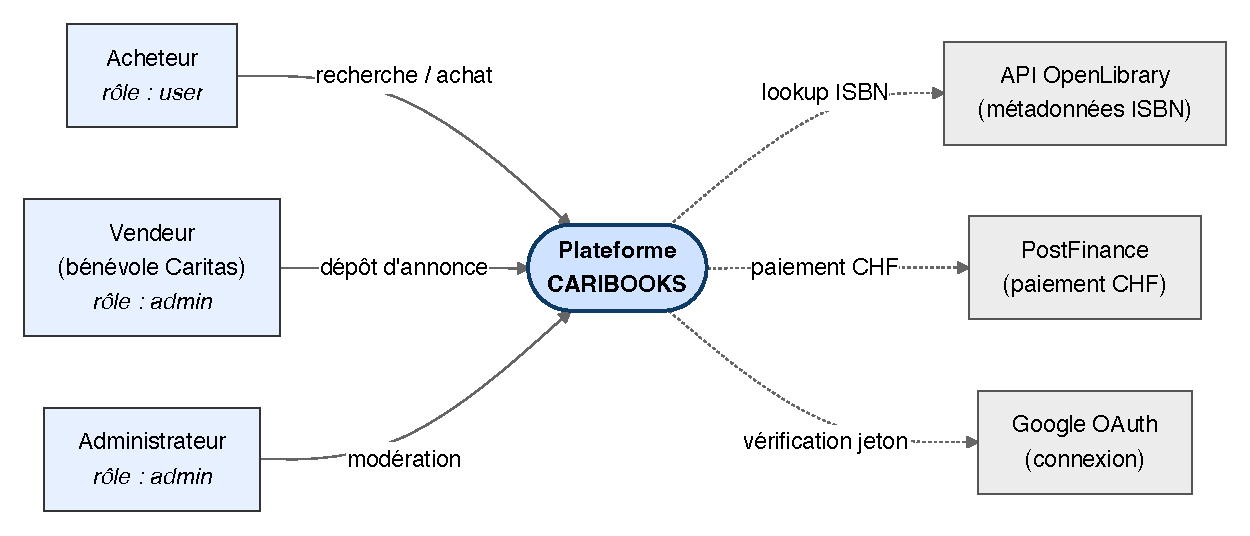
\includegraphics[width=\linewidth,keepaspectratio]{diagrams/contexte.pdf}
    \end{center}
    \column{0.50\textwidth}
    \begin{block}{Critères de succès du MVP --- mesurables}
      \begin{itemize}\small
        \item Mettre un livre en vente en \textbf{$<$ 2 minutes}
        \item Paiement \textbf{CHF natif} (TWINT, Visa/MC)
        \item \textbf{Livraison restreinte à la Suisse}
        \item Interface utilisable \textbf{sans formation}
      \end{itemize}
    \end{block}
    \vspace{6pt}
    \begin{exampleblock}{\small Ce qui est resté hors périmètre --- et assumé}
      \begin{itemize}\small
        \item Messagerie, favoris, avis : \textbf{backlog}, pas le MVP
        \item Un seul dépôt Caritas, pas de multi-boutique
      \end{itemize}
    \end{exampleblock}
  \end{columns}
\end{frame}

\section{État de l\textquotesingle{}art et choix technique}

\begin{frame}{Solutions existantes -- Pourquoi développer sur mesure ?}
  \begin{center}
  \small
  \renewcommand{\arraystretch}{1.4}
  \begin{tabular}{@{}lcccccc@{}}
    \toprule
    \textbf{Solution} & \textbf{Devise CHF} & \textbf{Scan ISBN}
      & \textbf{Back-office} & \textbf{Coût} & \textbf{Personnali\-sable} \\
    \midrule
    Momox       & \nomark  & \yes & \nomark     & Gratuit & \nomark \\
    Vinted      & \nomark  & \nomark  & Partiel & Gratuit & \nomark \\
    Shopify     & \yes & \nomark  & \yes    & Élevé   & Partiel \\
    WooCommerce & \yes & \nomark  & \nomark     & Moyen   & \yes \\
    Ricardo.ch  & \yes & \nomark  & \nomark     & Moyen   & \nomark \\
    \midrule
    \rowcolor{mybluepale}
    \textbf{CARIBOOKS} & \textbf{\yes} & \textbf{\yes} & \textbf{\yes}
      & \textbf{Faible} & \textbf{\yes\; Total} \\
    \bottomrule
  \end{tabular}
  \end{center}
  \vspace{4pt}
  \begin{columns}[T]
    \column{0.48\textwidth}
    \begin{alertblock}{\small Le vrai bloquant : aucune ligne ne coche tout}
      \begin{itemize}\small
        \item Shopify cocherait presque tout\ldots\ à $\approx$ 400 CHF/an d'abonnement
        \item \ldots\ pour une association qui vend des livres à 9 CHF
        \item WooCommerce : gratuit, mais back-office hors de portée d'un bénévole
      \end{itemize}
    \end{alertblock}
    \column{0.48\textwidth}
    \begin{exampleblock}{\small Ce que le sur-mesure coûte --- et que j'assume}
      \begin{itemize}\small
        \item Pas de support éditeur : la maintenance est \textbf{à ma charge}
        \item Sécurité et conformité à implémenter \textbf{soi-même}
        \item Contrepartie : \textbf{zéro} abonnement, et le tunnel CHF sous contrôle
      \end{itemize}
    \end{exampleblock}
  \end{columns}
\end{frame}

\begin{frame}{Stack technique --- Les choix, et pourquoi je les ai faits}
  \begin{block}{Justifications des choix}
    \begin{itemize}\small
      \item \tech{FastAPI} : performances ASGI, Pydantic auto, Swagger natif
      \item \tech{Next.js} : SSR pour le SEO vitrine, SPA pour le back-office
      \item \tech{MySQL} + \tech{SQLAlchemy} : relationnel éprouvé, transactions ACID, requêtes \textbf{paramétrées}
      \item \tech{SQL vs NoSQL} : besoin fondamentalement relationnel (FK, intégrité stock/commande)
      \item \tech{PostFinance} : paiement suisse en CHF --- détails à l'étape paiement
      \item \tech{GitHub Actions} + \tech{Vercel} : tests $\rightarrow$ déploiement continu
    \end{itemize}
  \end{block}
  \vspace{4pt}
\end{frame}

\begin{frame}{Architecture en couches --- Diagramme}
  \begin{center}
  \vspace{-4pt}
  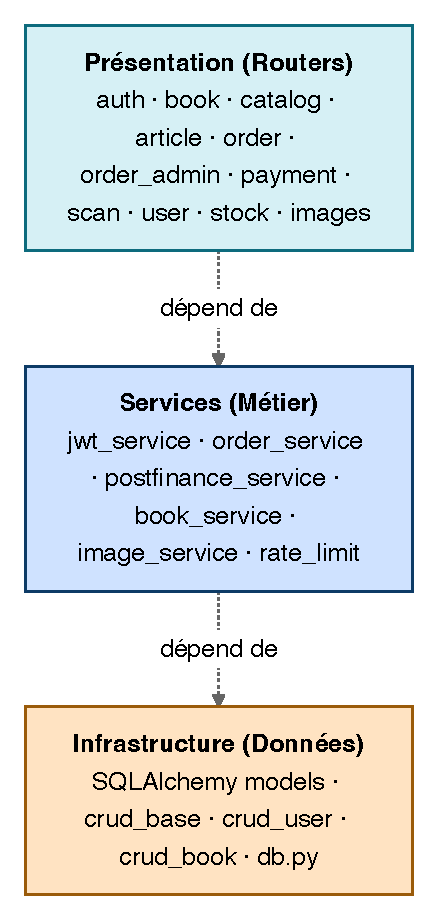
\includegraphics[width=\linewidth,height=0.82\textheight,keepaspectratio]{diagrams/architecture_couches.pdf}
  \end{center}
\end{frame}

\section{Gestion de projet}

\begin{frame}{Gestion de projet --- Kanban en continu \& environnement}
  \begin{columns}[T]
    \column{0.42\textwidth}
    \begin{block}{Méthodologie Agile Kanban}
      \begin{itemize}\small
        \item \textbf{Flux continu}, soirées de dev \textbf{17h--20h}
        \item Suivi : \textbf{Microsoft Planner} (Kanban)
        \item \textbf{Product Owner} : bénévole Caritas
        \item Démos au fil de l'avancement
      \end{itemize}
    \end{block}
    \vspace{5pt}
    \begin{center}
    \begin{tikzpicture}[every node/.style={font=\tiny}]
      \node[tag,fill=myblue,minimum width=5.4cm,text width=5.0cm,align=left]
        at (0, 0.00) {\textbf{Fondations} \; Env. GitHub/CI -- BDD -- Modélisation};
      \node[tag,fill=myblue,minimum width=5.4cm,text width=5.0cm,align=left]
        at (0,-0.54) {\textbf{Cœur fonctionnel} \; Auth -- Paiement -- Back-office v1};
      \node[tag,fill=myblue,minimum width=5.4cm,text width=5.0cm,align=left]
        at (0,-1.08) {\textbf{Fiabilisation \& sécurité} \; Durcissement -- Refactor -- CI};
      \node[tag,fill=myblue,minimum width=5.4cm,text width=5.0cm,align=left]
        at (0,-1.62) {\textbf{Consolidation admin} \; Statuts commande -- Nettoyage};
      \node[tag,fill=mysuccess,minimum width=5.4cm,text width=5.0cm,align=left]
        at (0,-2.16) {\textbf{Documentation \& certification} \; Dossier CDA -- Diagrammes -- Mémoire};
    \end{tikzpicture}
    \end{center}
    \column{0.55\textwidth}
    \begin{block}{Environnement de travail}
      \begin{itemize}\small
        \item \textbf{macOS} + VS Code / Copilot, Git/GitHub
        \item Backend : venv Python 3.12 (\texttt{requirements.txt} épinglé)
        \item Frontend : Node.js / npm
        \item Tests API manuels : \textbf{Thunder Client} ; doc : \textbf{Swagger UI}
        \item Diagrammes : Mermaid CLI, rendu PDF versionné
      \end{itemize}
    \end{block}
    \vspace{5pt}
    \begin{exampleblock}{\small Adapté au projet}
      \begin{itemize}\small
        \item Configuré dès la phase 1
        \item \texttt{startapp.sh} : backend + frontend en une commande
      \end{itemize}
    \end{exampleblock}
    \vspace{5pt}
    \begin{center}
    \badgegreen{5/5 phases livrées}\quad\badge{Déployé en ligne}
    \end{center}
  \end{columns}
\end{frame}

\section{Analyse et conception}

\begin{frame}{Cas d'utilisation --- trois profils, mais combien de rôles ?}
  \begin{columns}[T]
    \column{0.60\textwidth}
    \begin{center}
    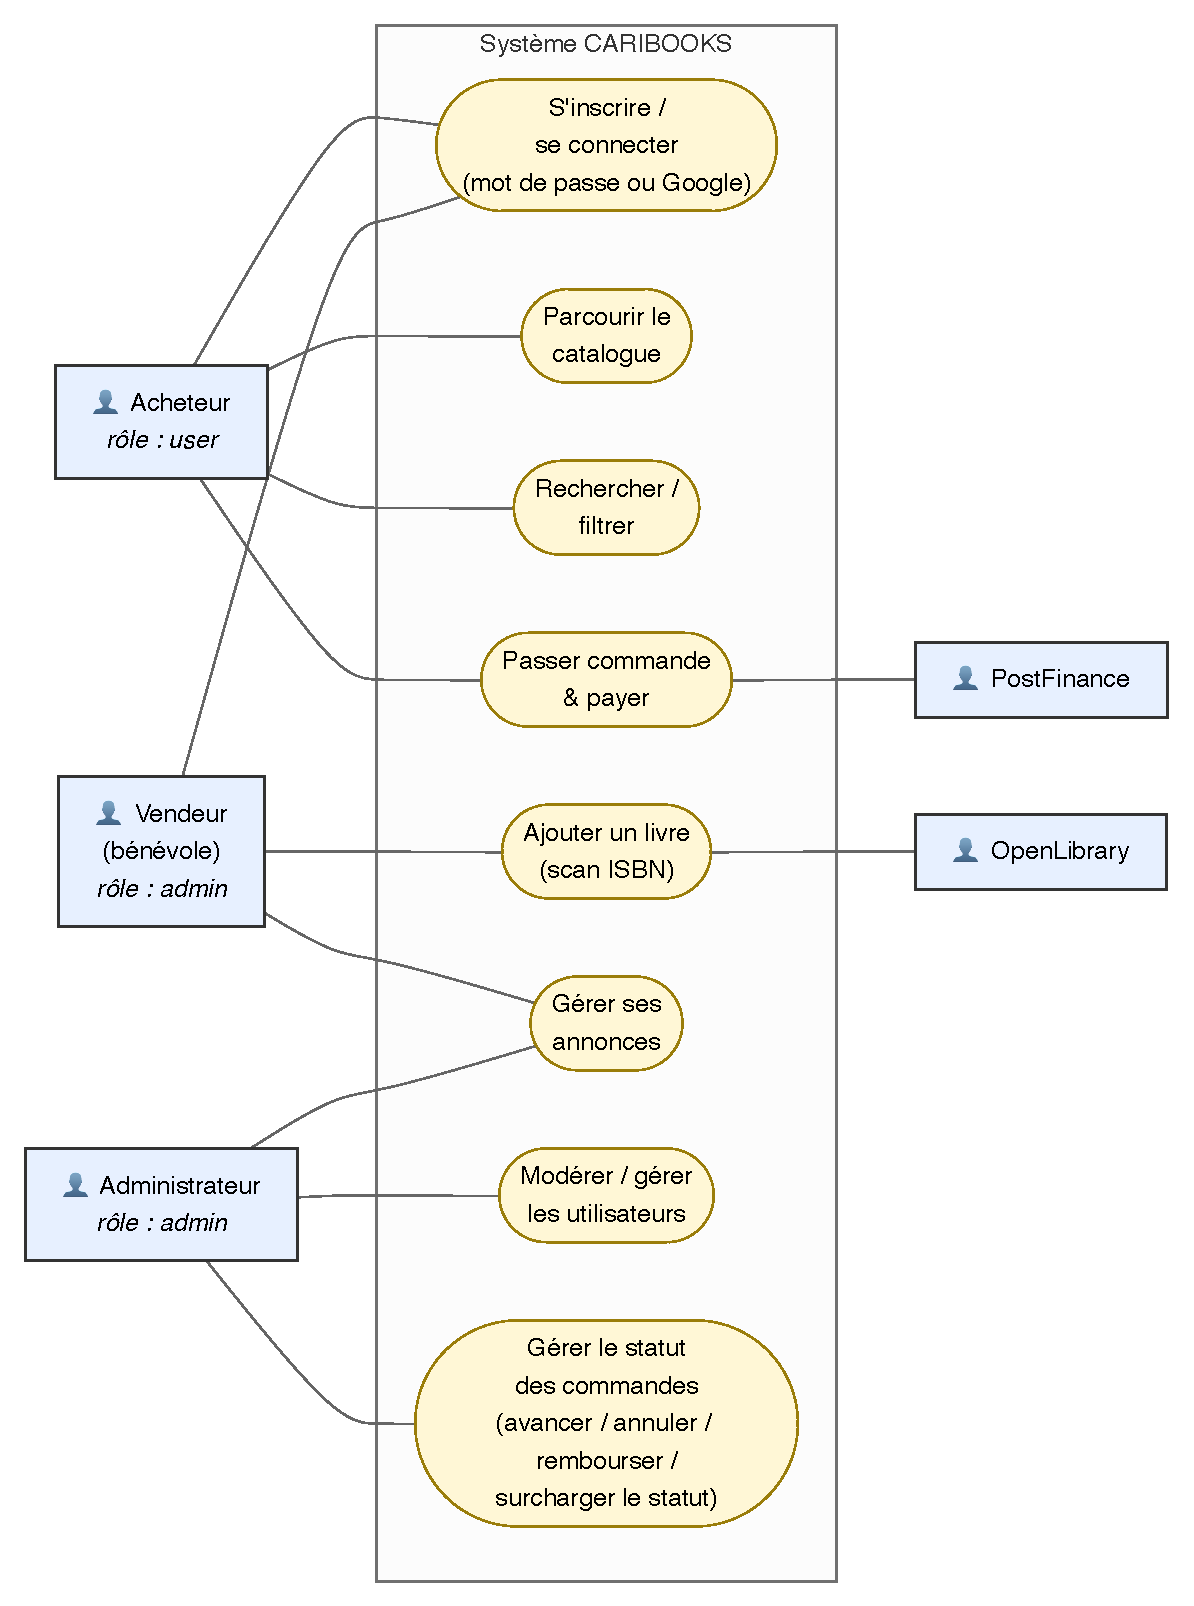
\includegraphics[width=\linewidth,height=0.78\textheight,keepaspectratio]{diagrams/use_case_global.pdf}
    \end{center}
    \column{0.36\textwidth}
    \begin{alertblock}{\small Le piège du \og\ un profil = un rôle \fg{}}
      \begin{itemize}\small
        \item \textbf{Bénévole} --- ajoute du stock
        \item \textbf{Administrateur} --- modère et suit
        \item \textbf{Acheteur} --- achète en CHF
      \end{itemize}
    \end{alertblock}
    \vspace{4pt}
    \begin{exampleblock}{\small Décision}
      \begin{itemize}\small
        \item[$\Rightarrow$] \textbf{2 rôles} : \texttt{admin} et \texttt{user}
        \item Bénévole et admin partagent \texttt{admin} : mêmes droits réels
        \item Un 3\textsuperscript{e} rôle sans droit distinct = complexité gratuite
      \end{itemize}
    \end{exampleblock}
  \end{columns}
\end{frame}

\begin{frame}{Modèle de données --- Architecture en héritage de table}
  \begin{columns}[T]
    \column{0.48\textwidth}
    \begin{block}{11 tables MySQL}
      \begin{itemize}\small
        \item \texttt{article} / \texttt{livre} : héritage 1-1 \textit{(clé primaire partagée)}
        \item \texttt{etat\_usure}, \texttt{type\_objet}
        \item \texttt{stock}, \texttt{source\_stock}
        \item \texttt{utilisateur}, \texttt{commande}
        \item \texttt{ligne\_commande}, \texttt{paiement}
        \item \texttt{scan\_isbn} (traçabilité des scans)
      \end{itemize}
    \end{block}
    \column{0.48\textwidth}
    \begin{alertblock}{\small Pourquoi une table \texttt{type\_objet} plutôt qu'un simple champ \og livre/DVD \fg{} ?}
      \begin{itemize}\small
        \item \texttt{livre} étend \texttt{article} par clé primaire partagée (\textit{Table Per Class})
        \item Un admin ajoute un nouveau type (DVD, jeu\ldots) via l'API, \textbf{sans redéploiement}
      \end{itemize}
    \end{alertblock}
    \vspace{4pt}
    \begin{exampleblock}{Index de performance}
      \scriptsize
      \texttt{idx\_livre\_isbn}, \texttt{idx\_stock\_article},
      \texttt{idx\_commande\_utilisateur}\ldots
    \end{exampleblock}
  \end{columns}
\end{frame}

\begin{frame}{Modèle de données — Diagramme}
  \begin{center}
  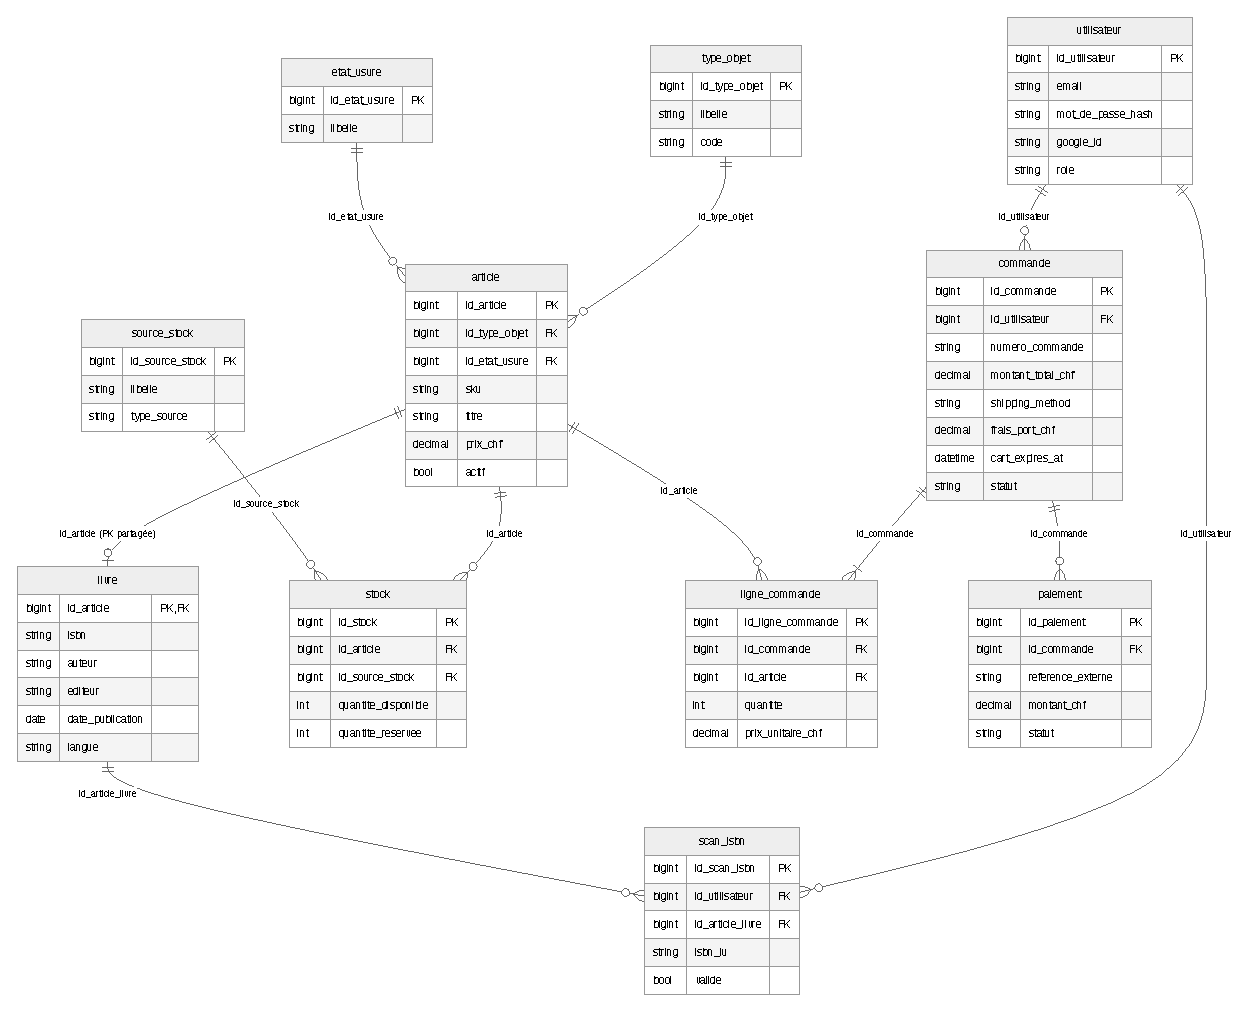
\includegraphics[width=\linewidth,height=0.82\textheight,keepaspectratio]{diagrams/mld.pdf}
  \end{center}
\end{frame}

\section{Le parcours d'un livre}

\begin{frame}{Notre fil rouge --- un exemplaire, une trajectoire complète}
  \begin{columns}[T]
    \column{0.5\textwidth}
    \begin{exampleblock}{Le livre que nous allons suivre}
      \begin{itemize}\small
        \item \textit{Divergente --- tome 2 : L'Insurrection}, Veronica Roth
        \item ISBN \texttt{978-2-266-27451-7}
        \item Déposé en rayon par un donateur, invendu depuis des semaines
      \end{itemize}
    \end{exampleblock}
    \vspace{6pt}
    \begin{block}{Ce que ça va couvrir}
      \begin{itemize}\small
        \item L'authentification (le bénévole doit se connecter)
        \item Le scan ISBN et le préremplissage OpenLibrary
        \item Son apparition au catalogue
        \item Son achat et son paiement en CHF
        \item Sa livraison et la clôture de la commande
      \end{itemize}
    \end{block}
    \column{0.44\textwidth}
    \begin{center}
    \begin{tikzpicture}[every node/.style={font=\scriptsize}, node distance=9mm]
      \node[tag,minimum width=4.2cm] (a) {1. Scan par le bénévole};
      \node[tag,below=of a,minimum width=4.2cm] (b) {2. Apparition au catalogue};
      \node[tag,below=of b,minimum width=4.2cm] (c) {3. Achat \& paiement CHF};
      \node[tag,below=of c,minimum width=4.2cm] (d) {4. Stock \& livraison};
      \node[taggreen,below=of d,minimum width=4.2cm] (e) {5. Clôture par l'admin};
      \draw[flow] (a)--(b); \draw[flow] (b)--(c);
      \draw[flow] (c)--(d); \draw[flow] (d)--(e);
    \end{tikzpicture}
    \end{center}
    \vspace{4pt}
  \end{columns}
\end{frame}

\begin{frame}{Avant toute chose --- le bénévole doit se connecter}
  \begin{columns}[T]
    \column{0.5\textwidth}
    \begin{block}{Connexion classique --- JWT}
      \begin{itemize}\small
        \item \texttt{POST /auth/token} $\Rightarrow$ hash \textbf{bcrypt} (rounds=12) vérifié
        \item JWT \textbf{HS256}, \texttt{\{sub, role, exp: 480 min\}}
        \item \texttt{get\_current\_user} / \texttt{require\_admin} : dépendances FastAPI sur chaque route protégée
      \end{itemize}
    \end{block}
    \vspace{4pt}
    \begin{alertblock}{\small Que se passe-t-il si \texttt{SECRET\_KEY} n'est pas définie ?}
      \begin{itemize}\small
        \item Valeur \og placeholder \fg{} connue $\Rightarrow$ l'application \textbf{refuse de démarrer}
        \item Absente $\Rightarrow$ clé aléatoire générée pour le processus (jamais de secret devinable)
      \end{itemize}
    \end{alertblock}
    \column{0.46\textwidth}
    \begin{block}{Connexion via Google --- second flux}
      \begin{itemize}\small
        \item \texttt{POST /auth/google} : jeton revérifié \textbf{côté serveur}
        \item Jamais de confiance aveugle envers le frontend
        \item Compte retrouvé/lié par \texttt{google\_id}, sinon créé
      \end{itemize}
    \end{block}
    \vspace{4pt}
    \begin{alertblock}{\small Pourquoi vérifier \texttt{email\_verified} ?}
      \begin{itemize}\small
        \item Faux $\Rightarrow$ connexion refusée (400)
        \item Sinon : prise de contrôle de compte possible
      \end{itemize}
    \end{alertblock}
  \end{columns}
\end{frame}

\begin{frame}{Authentification --- Diagramme de séquence (mot de passe + Google)}
  \begin{center}
  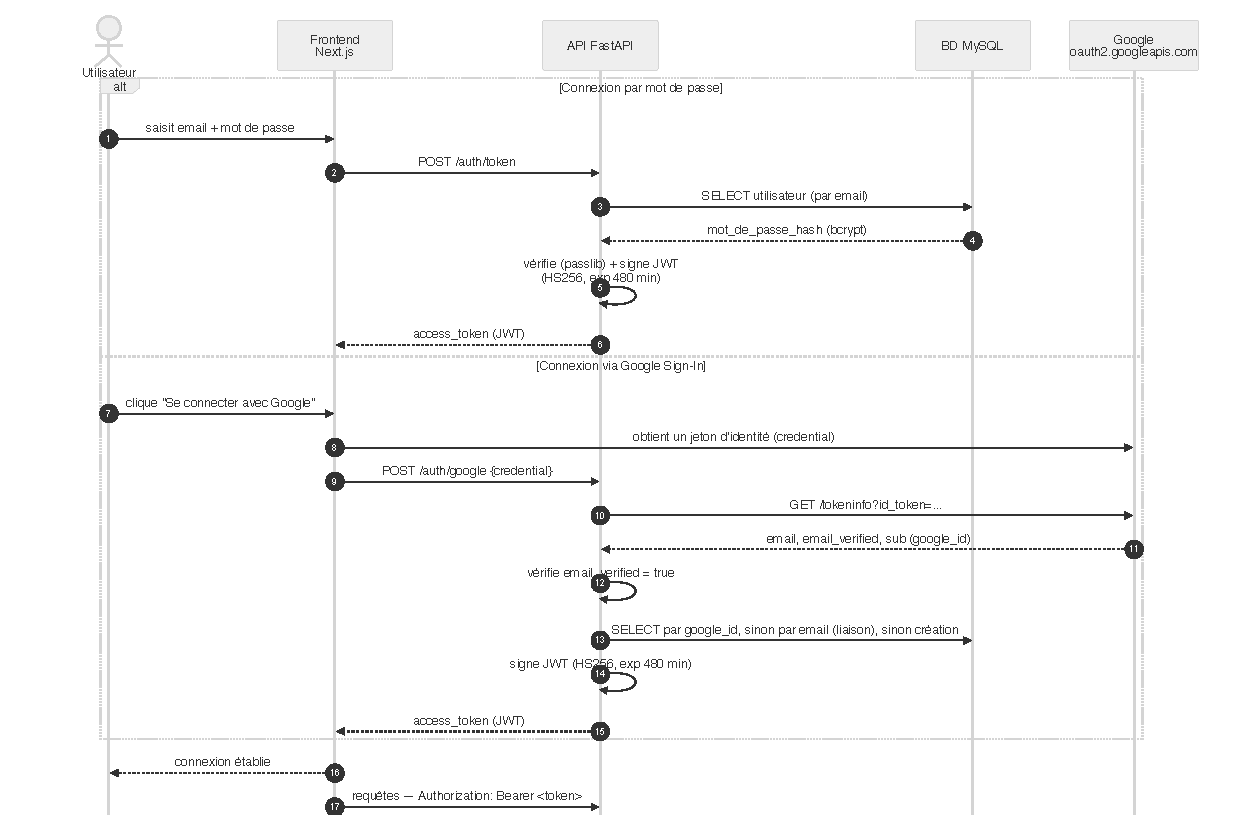
\includegraphics[width=\linewidth,height=0.82\textheight,keepaspectratio]{diagrams/sequence_auth.pdf}
  \end{center}
\end{frame}

\begin{frame}{Étape 1 --- Maquette mobile et flux d'ajout ($<$ 2 min)}
  \etapelivre{1}{scan et préremplissage automatique}
  \begin{columns}[T]
    \column{0.40\textwidth}
  \begin{center}
  \resizebox{!}{0.50\textheight}{%
  \begin{tikzpicture}
    \fill[gray!30] (0.8,0) rectangle (4.4,7.5);
    \fill[gray!30,rounded corners=6pt] (0.8,0) rectangle (4.4,7.5);
    \fill[white] (1.0,0.5) rectangle (4.2,7.0);
    \fill[black!85] (1.0,5.2) rectangle (4.2,7.0);
    \draw[myaccent,line width=1.2pt]
      (1.4,5.5) -- (1.4,5.2) -- (1.7,5.2);
    \draw[myaccent,line width=1.2pt]
      (3.8,5.5) -- (3.8,5.2) -- (3.5,5.2);
    \draw[myaccent,line width=1.2pt]
      (1.4,6.7) -- (1.4,7.0) -- (1.7,7.0);
    \draw[myaccent,line width=1.2pt]
      (3.8,6.7) -- (3.8,7.0) -- (3.5,7.0);
    \draw[myaccent!80,line width=0.8pt] (1.1,6.1) -- (4.1,6.1);
    \node[font=\tiny,text=white] at (2.6,6.4) {Ajouter un livre};
    \fill[mybluepale] (1.1,4.6) rectangle (4.1,5.1);
    \node[font=\tiny] at (2.6,4.85) {Titre : \textit{Divergente T.2 (prérempli)}};
    \fill[mybluepale] (1.1,4.0) rectangle (4.1,4.5);
    \node[font=\tiny] at (2.6,4.25) {Auteur : \textit{Veronica Roth (prérempli)}};
    \fill[gray!15] (1.1,3.4) rectangle (4.1,3.9);
    \node[font=\tiny] at (2.6,3.65) {État : Bon état \quad Prix : 9.50 CHF};
    \fill[mysuccess] (1.3,2.7) rectangle (3.9,3.2);
    \node[font=\tiny\bfseries,text=white] at (2.6,2.95) {Publier l'annonce};
    \fill[gray!50,rounded corners=2pt] (2.1,0.2) rectangle (3.1,0.35);
  \end{tikzpicture}}
  \end{center}
    \textcolor{mygray}{\scriptsize\textbf{RGAA} : libellés explicites, bouton $\geq$ 44px, saisie manuelle possible}
    \column{0.58\textwidth}
    \begin{center}
    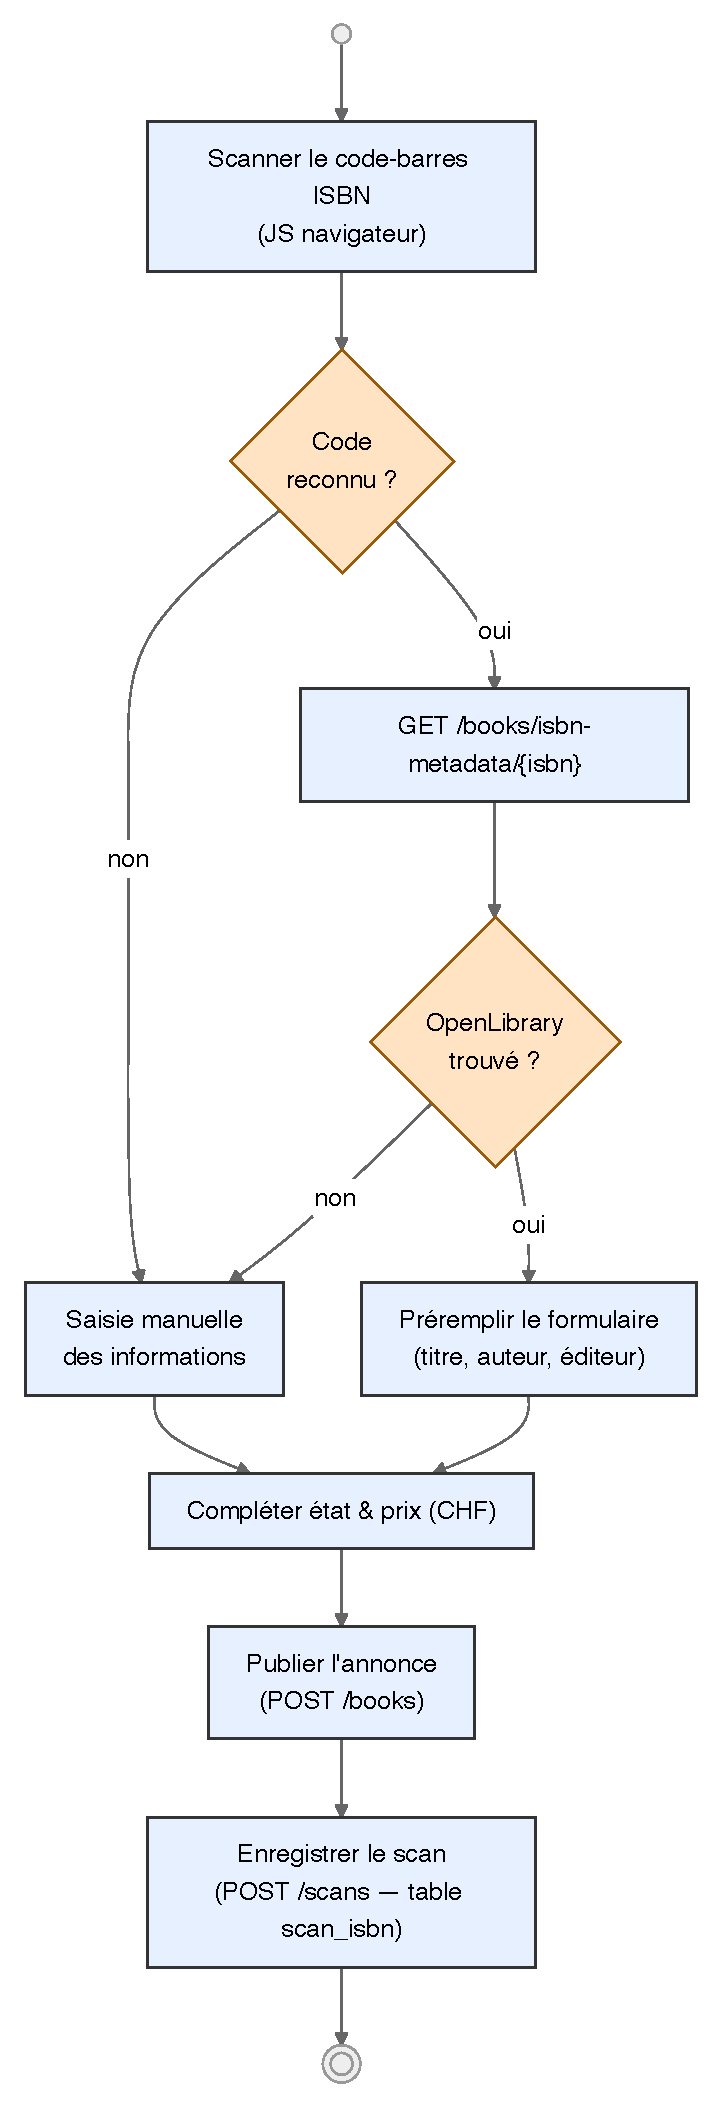
\includegraphics[width=\linewidth,height=0.68\textheight,keepaspectratio]{diagrams/activites_isbn.pdf}
    \end{center}
  \end{columns}
\end{frame}

\begin{frame}[fragile]{Étape 1 --- Le bénévole scanne notre \textit{Divergente}}
  \etapelivre{1}{scan et préremplissage automatique}
\begin{lstlisting}[style=pysmall,caption={}]
# presentation/book_router.py
@router.get("/isbn-metadata/{isbn}")
def get_isbn_metadata(isbn: str):
    clean = isbn.strip().upper().replace("-", "")

    # Source unique : OpenLibrary
    r = httpx.get(
        "https://openlibrary.org/api/books",
        params={"bibkeys": f"ISBN:{clean}",
                "format": "json",
                "jscmd":  "data"},
        timeout=8)
    if r.status_code == 200:
        book = r.json().get(f"ISBN:{clean}")
        if book and book.get("title"):
            return book  # "Divergente - tome 2", Roth...

    raise HTTPException(404, "ISBN introuvable")
\end{lstlisting}
\end{frame}

\begin{frame}{Étape 2 --- Notre livre apparaît au catalogue}
  \etapelivre{2}{visible et trouvable}
  \begin{center}
  \resizebox{!}{0.56\textheight}{%
  \begin{tikzpicture}
    \fill[gray!20] (0,5.4) rectangle (6,6.0);
    \fill[white!90!gray] (0.1,5.45) circle (0.08);
    \fill[white!90!gray] (0.3,5.45) circle (0.08);
    \fill[white!90!gray] (0.5,5.45) circle (0.08);
    \fill[white] (0.8,5.35) rectangle (5.2,5.6);
    \node[font=\tiny,text=mygray] at (3,5.475) {caribooks.vercel.app};
    \draw[myblue,thick] (0,0) rectangle (6,5.4);
    \fill[myblue] (0,4.9) rectangle (6,5.4);
    \node[font=\tiny\bfseries,text=white] at (1,5.15) {CARIBOOKS};
    \node[font=\tiny,text=white] at (3,5.15) {Catalogue \quad Connexion};
    \fill[gray!15] (0.3,4.5) rectangle (5.7,4.8);
    \node[font=\tiny,text=mygray] at (3,4.65) {Rechercher un livre...};
    \fill[mybluepale] (0.3,4.1) rectangle (1.6,4.35);
    \fill[mybluepale] (1.7,4.1) rectangle (3.0,4.35);
    \fill[mybluepale] (3.1,4.1) rectangle (4.4,4.35);
    \node[font=\tiny] at (0.95,4.225) {Trier par};
    \node[font=\tiny] at (2.35,4.225) {État};
    \node[font=\tiny] at (3.75,4.225) {Prix CHF};
    \foreach \x/\ti/\p in {0.3/Roth/9.50, 2.3/Orwell/15.00, 4.3/St-Exupery/8.50} {
      \fill[gray!10] (\x,2.4) rectangle ({\x+1.7},{3.9});
      \fill[mybluepale!80] (\x,2.4) rectangle ({\x+1.7},{3.3});
      \node[font=\tiny\bfseries,align=center,text width=14mm] at ({\x+0.85},2.85) {\ti};
      \fill[mysuccess] (\x,2.1) rectangle ({\x+1.7},{2.4});
      \node[font=\tiny,text=white] at ({\x+0.85},2.25) {\p\,CHF};
    }
    \fill[myblue!80] (0,0) rectangle (6,0.5);
    \node[font=\tiny,text=white] at (3,0.25) {Livraison Suisse uniquement \textbullet{} Paiement CHF};
    \draw[myaccent,thick,-{Stealth[length=2mm]}] (1.15,1.7) -- (1.15,2.05);
    \node[font=\tiny\bfseries,text=myaccent] at (1.15,1.5) {notre livre};
  \end{tikzpicture}}
  \end{center}
  \textcolor{mygray}{\scriptsize\textbf{RGAA}}
  \begin{itemize}\scriptsize
    \item \textcolor{mygray}{Contraste $\geq$ 4.5:1 sur les prix}
    \item \textcolor{mygray}{Zones cliquables $\geq$ 44px}
    \item \textcolor{mygray}{Focus clavier cohérent}
  \end{itemize}
\end{frame}

\begin{frame}[fragile]{Étape 2 --- Le piège du N+1 sur le catalogue}
  \etapelivre{2}{visible et trouvable}
  \begin{columns}[T]
    \column{0.46\textwidth}
    \begin{alertblock}{\small Le symptôme}
      \begin{itemize}\small
        \item Chaque vignette voulait savoir \og\ reste-t-il un exemplaire ? \fg{}
        \item Le front récupérait \textbf{toute} la table \texttt{stock}\ldots\ une fois \textbf{par livre}
        \item 60 livres $\Rightarrow$ 60 requêtes qui rapatrient la même chose
      \end{itemize}
    \end{alertblock}
    \vspace{4pt}
    \begin{exampleblock}{\small La correction}
      \begin{itemize}\small
        \item \textbf{Un seul} endpoint, \textbf{une seule} requête \texttt{GROUP BY}
        \item Calcul déplacé \textbf{côté SQL}, pas côté JavaScript
        \item Appelé depuis un \textbf{Server Component} : le navigateur ne fait rien
      \end{itemize}
    \end{exampleblock}
    \column{0.52\textwidth}
\begin{lstlisting}[style=pysmall,caption={}]
# presentation/stock_router.py
@router.get("/availability",
            response_model=dict[int, int])
def stock_availability(db: DbSession,
                       article_ids: str | None = None):
    q = db.query(
        models.Stock.id_article,
        func.sum(models.Stock.quantite_disponible
                 - models.Stock.quantite_reservee),
    )
    rows = q.group_by(models.Stock.id_article).all()
    return {int(a): max(0, int(t or 0))
            for a, t in rows}
\end{lstlisting}
    \begin{block}{\small Ce que ça dit de ma démarche}
      \begin{itemize}\small
        \item Le \textbf{disponible réel} = disponible $-$ réservé, jamais stocké en dur
        \item Une seule source de vérité, donc pas de désynchronisation possible
      \end{itemize}
    \end{block}
  \end{columns}
\end{frame}

\begin{frame}{Étape 3 --- Un client l'achète : le tunnel CHF PostFinance}
  \etapelivre{3}{achat et paiement en CHF}
  \begin{columns}[T]
    \column{0.48\textwidth}
    \begin{block}{Pourquoi PostFinance ?}
      \begin{itemize}\small
        \item \textbf{TWINT} natif (paiement mobile dominant CH)
        \item PostCard, Visa, Mastercard en \textbf{CHF}
        \item Acteur 100\% suisse, réglementation conforme
      \end{itemize}
    \end{block}
    \column{0.48\textwidth}
    \begin{block}{Sécurisation webhook}
      \begin{itemize}\small
        \item Signature \textbf{ECDSA} (\textit{Elliptic Curve Digital Signature Algorithm}) vérifiée avant mise à jour
        \item \texttt{with\_for\_update()} : verrou SQL --- accès concurrents
        \item Finalisation atomique de la commande
      \end{itemize}
    \end{block}
  \end{columns}
\end{frame}

\begin{frame}{Étape 3 --- Paiement : diagramme de séquence}
  \etapelivre{3}{achat et paiement en CHF}
  \begin{center}
  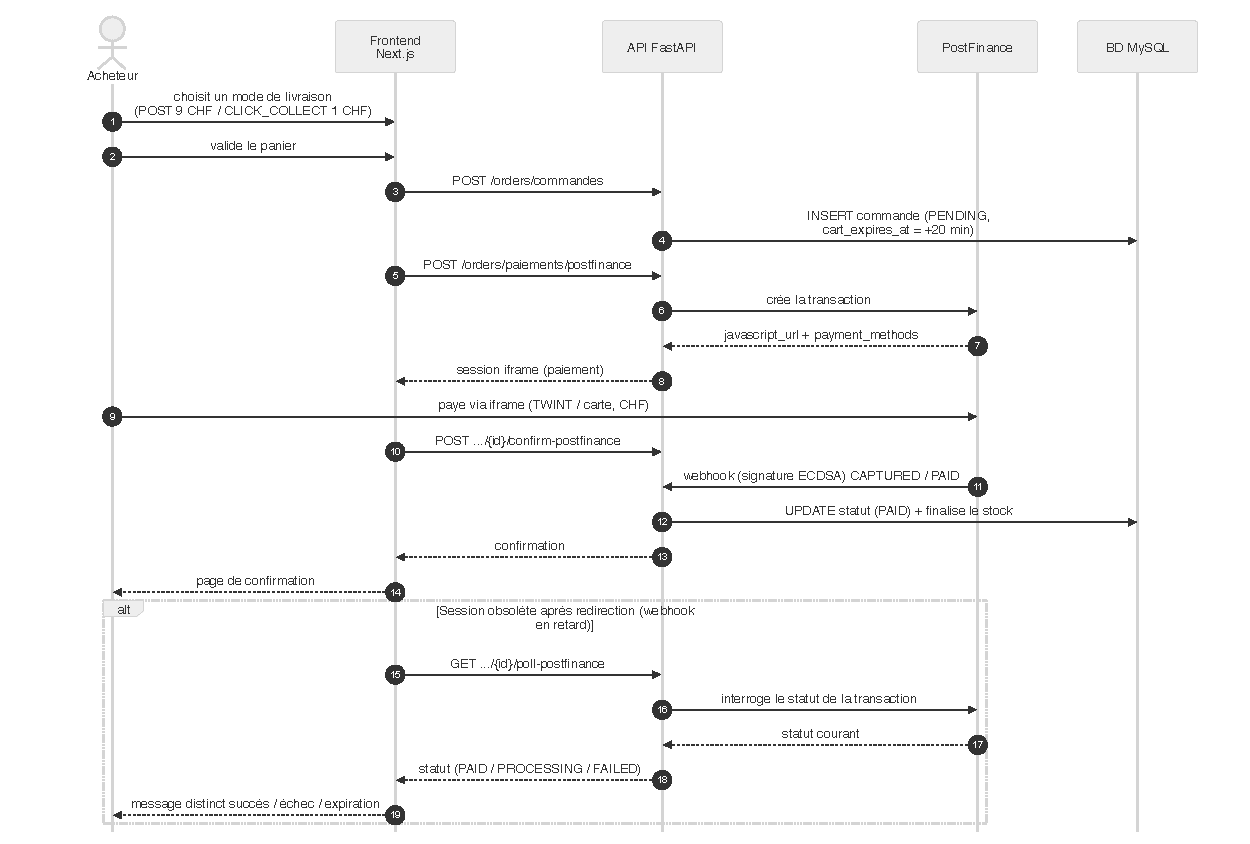
\includegraphics[width=\linewidth,height=0.76\textheight,keepaspectratio]{diagrams/sequence_paiement.pdf}
  \end{center}
\end{frame}

\begin{frame}{Démonstration en direct --- l'achat de notre livre}
  
  \vspace{6pt}
  \begin{columns}[T]
    \column{0.38\textwidth}
    \centering
    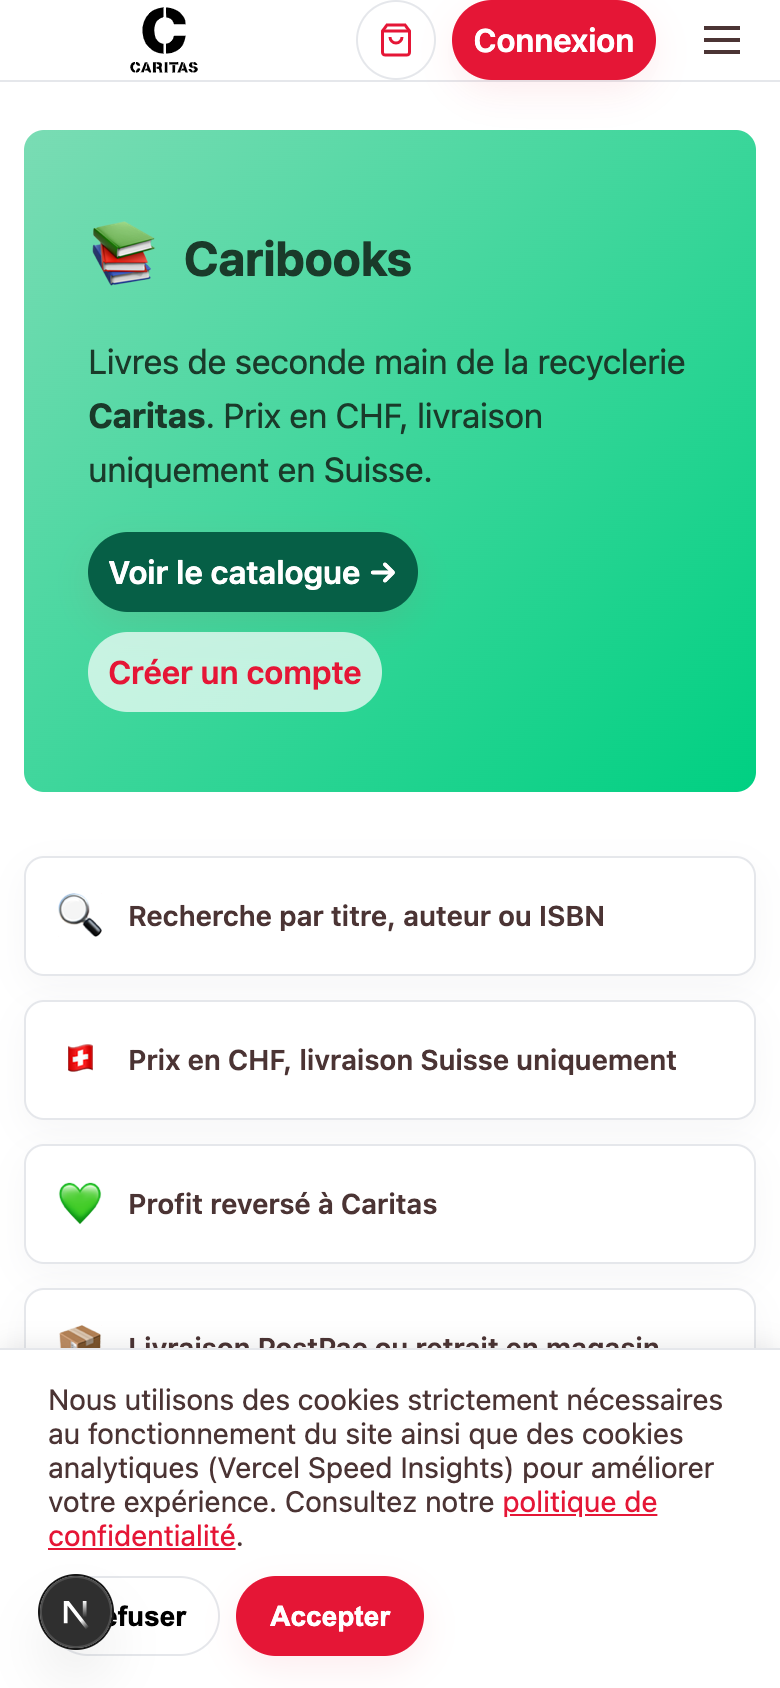
\includegraphics[height=0.52\textheight,keepaspectratio]{vue_telephone.png}\\
    \scriptsize\textit{Vitrine mobile}
    \column{0.60\textwidth}
    \centering
    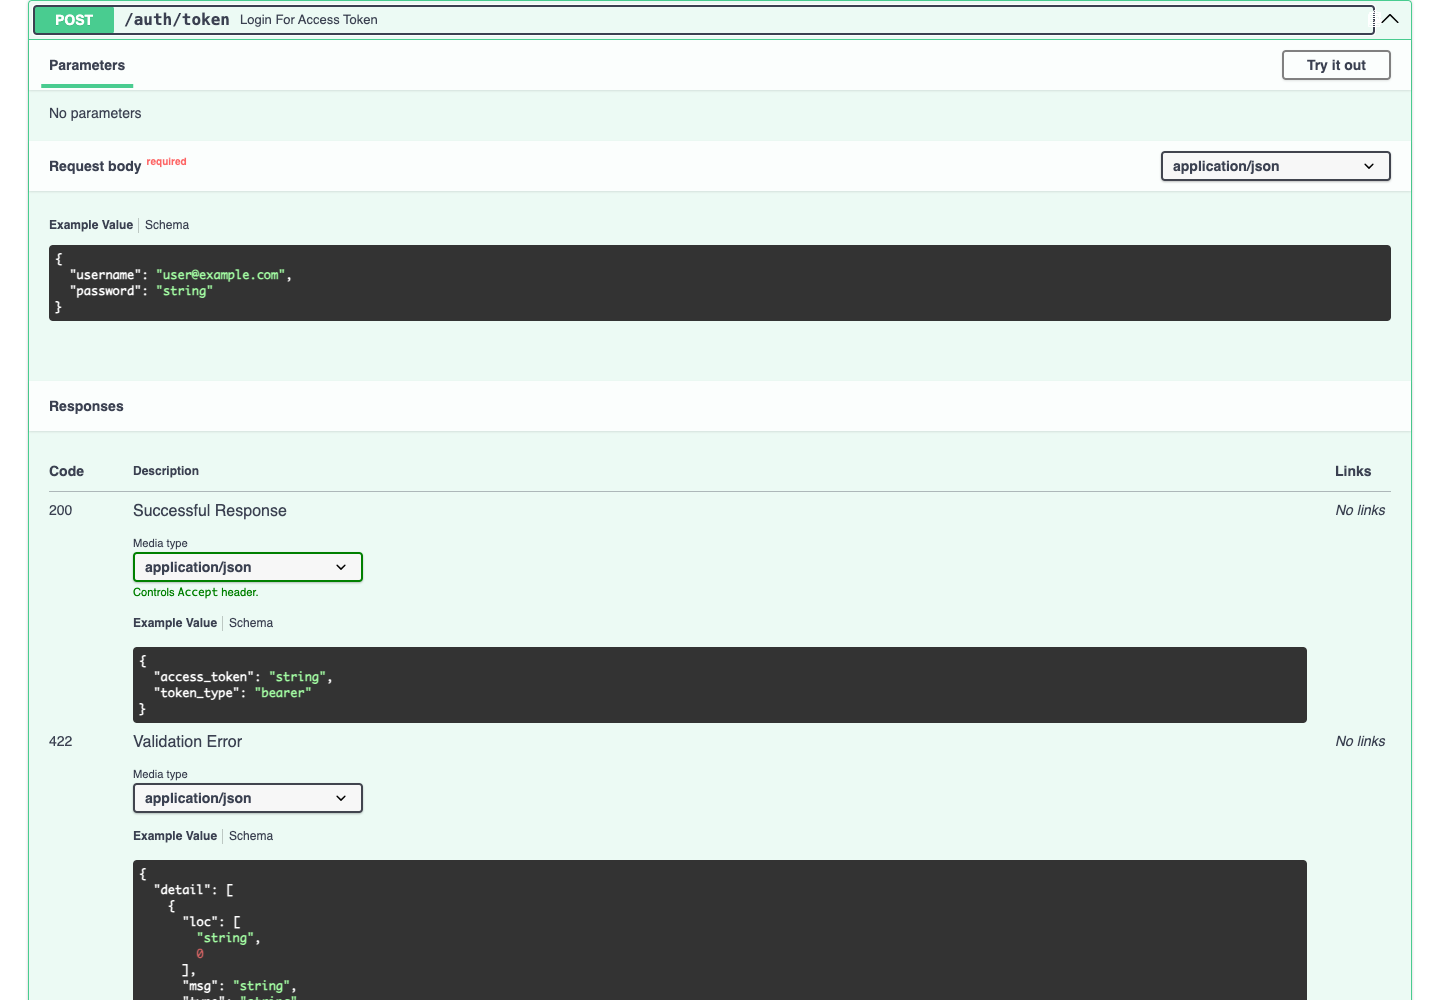
\includegraphics[height=0.42\textheight,keepaspectratio]{SWAGGER_LOGIN_DETAIL.png}\\
    \scriptsize\textit{Swagger --- POST /auth/token}
  \end{columns}
  \vspace{4pt}
\end{frame}

\begin{frame}[fragile]{Étape 4 --- Réserver le stock et choisir la livraison}
  \etapelivre{4}{stock et livraison}
  \begin{columns}[T]
    \column{0.46\textwidth}
    \begin{block}{Choix du mode de livraison}
      \begin{itemize}\small
        \item \texttt{POST} : envoi postal, \textbf{9 CHF}
        \item \texttt{CLICK\_COLLECT} : retrait en magasin, \textbf{1 CHF}
      \end{itemize}
    \end{block}
    \vspace{5pt}
    \begin{block}{Réservation temporaire de stock}
      \begin{itemize}\small
        \item Fenêtre de \textbf{20 minutes} (\texttt{cart\_expires\_at})
        \item Expiration $\Rightarrow$ relibération automatique
      \end{itemize}
    \end{block}
    \vspace{5pt}
    \begin{alertblock}{\small Que se passe-t-il si deux clients achètent le \textbf{dernier} exemplaire au même instant ?}
      \begin{itemize}\small
        \item Sans verrou : les deux lisent \og en stock \fg{} en même temps
        \item Conséquence : double vente du même exemplaire
      \end{itemize}
    \end{alertblock}
    \column{0.50\textwidth}
\begin{lstlisting}[style=pysmall,caption={}]
# services/order_service.py
SHIPPING_FEES_CHF = {
    "POST": 9.0,
    "CLICK_COLLECT": 1.0,
}

def _lock_stock_rows(db, ids_article):
    return db.query(models.Stock).filter(
        models.Stock.id_article.in_(ids_article)
    ).with_for_update().all()
\end{lstlisting}
    \begin{exampleblock}{\small Pourquoi \texttt{FOR UPDATE} ?}
      \begin{itemize}\small
        \item 2\textsuperscript{e} transaction attend, relit un stock à 0
        \item Atomicité garantie par MySQL/InnoDB, pas par le code applicatif
      \end{itemize}
    \end{exampleblock}
  \end{columns}
\end{frame}

\begin{frame}{Étape 5 --- L'association clôture la commande}
  \etapelivre{5}{suivi et clôture par l'admin}
  \begin{columns}[T]
    \column{0.42\textwidth}
    \begin{block}{\texttt{order\_admin\_router}}
      \begin{itemize}\small
        \item Avancer / annuler / rembourser
        \item Marquer \og envoyée \fg{} / \og à réception \fg{}
        \item Surcharge manuelle du statut (cas exceptionnels)
        \item Toutes les routes protégées par \texttt{require\_admin}
        \item Front \texttt{/admin} : non connecté $\Rightarrow$ redirection \texttt{/login} avec message
      \end{itemize}
    \end{block}
    \vspace{4pt}
    \begin{alertblock}{\small Qu'arrive-t-il si un client consulte la commande d'un autre ?}
      \begin{itemize}\small
        \item\textbf{404}, comme si elle n'existait pas
        \item Non-admin $\rightarrow$ \texttt{/orders/admin/*} : \textbf{403}
        \item Vérifié par un test dédié, \texttt{test\_orders\_cross\_user\_isolation}
      \end{itemize}
    \end{alertblock}
    \column{0.54\textwidth}
    \begin{center}
    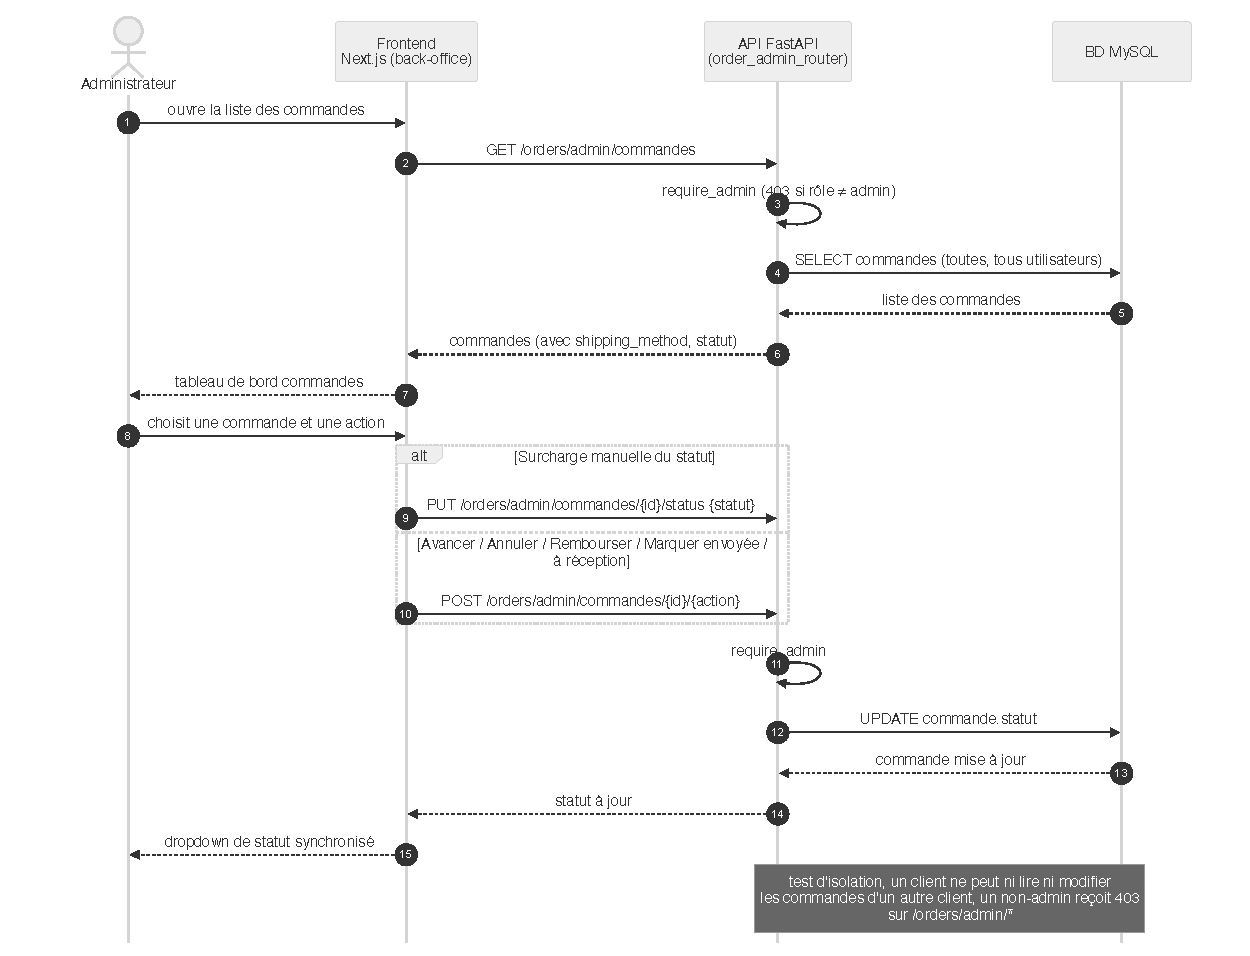
\includegraphics[width=\linewidth,height=0.62\textheight,keepaspectratio]{diagrams/sequence_admin_commande.pdf}
    \end{center}
  \end{columns}
\end{frame}

\begin{frame}[fragile]{Le bug le plus coûteux --- CORS, un proxy et une barre oblique}
  \begin{columns}[T]
    \column{0.47\textwidth}
    \begin{block}{\small Le montage : supprimer CORS plutôt que l'autoriser}
      \begin{itemize}\small
        \item Front Vercel et API Oracle Cloud = \textbf{deux origines}
        \item Next réécrit \texttt{/api/proxy/*} vers le backend
        \item Pour le navigateur, tout reste \textbf{same-origin} : plus de préflight
      \end{itemize}
    \end{block}
    \vspace{4pt}
    \begin{alertblock}{\small Le symptôme : la page admin \og Utilisateurs \fg{} restait vide}
      \begin{itemize}\small
        \item \texttt{Failed to fetch}, listes vides, \textbf{aucune} erreur serveur
        \item Reproductible en prod uniquement
      \end{itemize}
    \end{alertblock}
    \column{0.49\textwidth}
    \begin{exampleblock}{\small La chaîne causale --- 4 maillons}
      \begin{enumerate}\small
        \item Next normalise \texttt{/users/} $\rightarrow$ \texttt{/users} (\textbf{308}) \textit{avant} la réécriture
        \item Le proxy appelle donc le backend \textbf{sans} la barre oblique
        \item FastAPI \texttt{redirect\_slashes} renvoie un \textbf{307} vers une URL \textbf{absolue} du backend
        \item Redirection \textbf{cross-origin} $\Rightarrow$ le navigateur \textbf{supprime} l'en-tête \texttt{Authorization}
      \end{enumerate}
    \end{exampleblock}
    \vspace{3pt}
\begin{lstlisting}[style=pysmall,caption={}]
// next.config.js
skipTrailingSlashRedirect: true,
\end{lstlisting}
    \begin{block}{\small La leçon}
      \begin{itemize}\small
        \item Une requête \textbf{non authentifiée} n'est pas forcément une requête \textbf{refusée}
        \item Le coupable n'était ni le front, ni l'API, mais leur \textbf{contrat implicite}
      \end{itemize}
    \end{block}
  \end{columns}
\end{frame}

\begin{frame}{Difficultés rencontrées --- ce que j'ai appris en le faisant seul}
  \begin{itemize}\small
    \item \textbf{Backend Express.js $\rightarrow$ FastAPI} --- robustesse et validation automatique
    \item \textbf{Scan code-barres} --- latence et reconnaissance insuffisantes, algorithme revu
    \item \textbf{Paiement Payrexx $\rightarrow$ PostFinance} --- sandbox sans CB réelle
    \item \textbf{Gestion du périmètre} --- demandes récurrentes (favoris, chat) reportées au backlog
    \item \textbf{Formation + projet perso} --- développement en soirée, 3 j/semaine
    \item \textbf{Vercel + \texttt{output: standalone}} --- assets statiques en 404 en prod, option désormais conditionnée à la variable \texttt{VERCEL}
  \end{itemize}
  \vspace{6pt}
  \begin{exampleblock}{\small Gestion du commanditaire}
    \begin{itemize}\small
      \item Commanditaire qui redemande sans cesse de nouvelles fonctionnalités
      \item Chaque demande $\rightarrow$ backlog, jamais le travail en cours
      \item Le MVP restait la seule priorité contractuelle
    \end{itemize}
  \end{exampleblock}
\end{frame}

\section{Cybersécurité et qualité}

\begin{frame}{Cybersécurité --- Mesures implémentées (OWASP Top 10)}
  \begin{center}
  \small
  \renewcommand{\arraystretch}{1.35}
  \begin{tabular}{@{}p{3.8cm}p{3.4cm}p{4.2cm}@{}}
    \toprule
    \textbf{Menace / Risque} & \textbf{Mesure implémentée} & \textbf{Technologie} \\
    \midrule
    Injection SQL               & Requêtes paramétrées       & SQLAlchemy ORM \\
    Mots de passe compromis     & Hashage adaptatif (cost=12) & bcrypt / pwdlib \\
    Accès non autorisé          & Auth obligatoire routes     & JWT + HTTPBearer \\
    Élévation de privilèges     & Contrôle rôles strict       & \texttt{require\_admin} FastAPI \\
    Données invalides           & Validation schémas          & Pydantic + HTTPException \\
    Token intercepté            & Expiration + TLS prod       & JWT \texttt{exp}, HTTPS \\
    Secrets en clair            & Variables d'environnement   & \texttt{.env} + python-dotenv \\
    Race condition stock        & Verrou SQL transactionnel   & \texttt{with\_for\_update()} \\
    Non-conformité RGPD/nLPD    & Export + effacement + consentement & \texttt{/users/me}, bannière cookies \\
    Montant PostFinance falsifié & Vérification vs total commande avant finalisation & \texttt{amount\_matches\_commande} \\
    \bottomrule
  \end{tabular}
  \end{center}
\end{frame}

\begin{frame}[fragile]{Cybersécurité --- SSRF : quand l'API télécharge une URL fournie}
  \begin{columns}[T]
    \column{0.46\textwidth}
    \begin{alertblock}{\small L'admin colle une URL de couverture. Que peut-il viser ?}
      \begin{itemize}\small
        \item \texttt{http://169.254.169.254/} : métadonnées cloud $\Rightarrow$ \textbf{fuite de secrets}
        \item \texttt{http://127.0.0.1:3306} : MySQL en réseau privé
        \item Le serveur devient un \textbf{proxy} vers son propre VCN
      \end{itemize}
    \end{alertblock}
    \vspace{4pt}
    \begin{block}{\small Défense en profondeur}
      \begin{itemize}\small
        \item Résolution DNS, puis rejet de toute IP \textbf{privée / loopback / link-local}
        \item \textbf{SVG exclu} des formats acceptés : il embarque du \texttt{<script>}, donc XSS stocké depuis notre propre origine
        \item Taille et \texttt{Content-Type} vérifiés avant écriture
      \end{itemize}
    \end{block}
    \column{0.52\textwidth}
\begin{lstlisting}[style=pysmall,caption={}]
# services/image_service.py
def _resolve_pinned_ip(hostname: str) -> str:
    infos = socket.getaddrinfo(hostname, None)
    ips = {info[4][0] for info in infos}
    if not ips or not all(_is_public_ip(ip)
                          for ip in ips):
        raise ValueError("URL host is not allowed")
    return next(iter(ips))   # on se connecte a CETTE IP
\end{lstlisting}
    \begin{exampleblock}{\small Pourquoi \textbf{épingler} l'IP au lieu de revérifier l'URL ?}
      \begin{itemize}\small
        \item Sinon : \textbf{DNS rebinding} (TOCTOU)
        \item Le contrôle passe sur une IP publique à TTL très court\ldots
        \item \ldots\ et la connexion, une seconde plus tard, résout vers \texttt{127.0.0.1}
        \item Valider puis re-résoudre \textbf{ne valide rien}
      \end{itemize}
    \end{exampleblock}
  \end{columns}
\end{frame}

\begin{frame}{Veille technologique --- de la lecture à la décision}
  \begin{columns}[T]
    \column{0.44\textwidth}
    \begin{block}{Sources suivies}
      \begin{itemize}\small
        \item \textbf{OWASP Top 10} : référentiel principal
        \item \textbf{GitHub Dependabot} : alertes CVE automatiques
        \item \textbf{Documentation officielle} FastAPI / Next.js
        \item \textbf{Daily.dev} / bytes : newsletter tech hebdo
      \end{itemize}
    \end{block}
    \vspace{4pt}
    \begin{block}{Mesures complémentaires}
      \begin{itemize}\small
        \item CORS : origines autorisées (Vercel + localhost)
        \item En-têtes \textbf{CSP}, \texttt{X-Content-Type-Options}, \texttt{Referrer-Policy}
        \item \texttt{/static} monté pour les images (pas d'URL tiers)
      \end{itemize}
    \end{block}
    \column{0.52\textwidth}
    \begin{alertblock}{\small La veille ne sert à rien si elle ne change pas le code}
      \begin{itemize}\small
        \item La doc FastAPI a \textbf{changé de librairies} depuis mes premiers commits
        \item Relire la doc officielle m'a fait découvrir \textbf{deux dettes} invisibles
      \end{itemize}
    \end{alertblock}
    \vspace{4pt}
    \begin{center}
    \scriptsize
    \renewcommand{\arraystretch}{1.3}
    \begin{tabular}{@{}p{2.0cm}p{1.5cm}p{3.6cm}@{}}
      \toprule
      \textbf{Avant} & \textbf{Après} & \textbf{Pourquoi} \\
      \midrule
      \texttt{python-jose} & \texttt{PyJWT} & Non maintenue depuis 2021, retirée de la doc FastAPI \\
      \texttt{passlib} & \texttt{pwdlib} & Importe \texttt{crypt}, \textbf{supprimé de Python 3.13} \\
      \bottomrule
    \end{tabular}
    \end{center}
    \vspace{3pt}
    \begin{exampleblock}{\small Migration sans rupture}
      \begin{itemize}\small
        \item \textbf{bcrypt conservé} : les hashs existants restent valides, zéro migration de données
        \item 70/70 tests verts \textbf{après désinstallation} des deux anciennes librairies
      \end{itemize}
    \end{exampleblock}
  \end{columns}
\end{frame}

\begin{frame}{Données personnelles (RGPD / nLPD) \& Accessibilité}
  \begin{columns}[T]
    \column{0.5\textwidth}
    \begin{block}{Protection des données — RGPD / nLPD}
      \begin{itemize}\small
        \item Politique de confidentialité + CGU + bannière cookies
        \item Bases légales, durées de conservation, sous-traitants documentés
        \item \textbf{Portabilité} : \texttt{GET /users/me/export} (JSON)
        \item \textbf{Effacement} : \texttt{DELETE /users/me} --- anonymisation, commandes conservées
      \end{itemize}
    \end{block}
    \column{0.5\textwidth}
    \begin{block}{Accessibilité (WCAG / RGAA)}
      \begin{itemize}\small
        \item HTML sémantique (\texttt{header}/\texttt{nav}/\texttt{main}/\texttt{footer})
        \item \texttt{alt} sur les couvertures, \texttt{aria-label}/\texttt{aria-expanded}
        \item \texttt{label} associés + \texttt{aria-describedby} sur erreurs
        \item \texttt{prefers-reduced-motion}
      \end{itemize}
    \end{block}
    \vspace{4pt}
    \badgeorange{Audit RGAA complet : phase 2}
  \end{columns}
\end{frame}

\section{Tests et déploiement}

\begin{frame}{Tests et couverture --- 101/101, 78\,\%}
  \begin{columns}[T]
    \column{0.48\textwidth}
    \begin{block}{Stratégie de test à 3 niveaux}
      \begin{itemize}\small
        \item \textbf{Tests unitaires} : JWT, bcrypt, ISBN, calculs CHF, SSRF, rate limiting
        \item \textbf{Tests d'intégration} : \texttt{TestClient} FastAPI + MySQL, isolation inter-utilisateurs
        \item \textbf{Test fonctionnel E2E} : parcours achat complet
        \item \textbf{Sandbox PostFinance} : scénarios succès / échec
      \end{itemize}
    \end{block}
    \vspace{5pt}
    \badgegreen{101 / 101 tests passants (70 pytest + 31 Vitest)}
    \vspace{5pt}
    \begin{alertblock}{\small Ce qu'un test a réellement attrapé}
      \begin{itemize}\small
        \item \texttt{test\_orders\_cross\_user\_isolation} : un client lisait la commande d'un autre
        \item Corrigé en \textbf{404} (et non 403) : ne pas confirmer l'existence de la ressource
        \item Les lignes surlignées ci-contre restent mes \textbf{angles morts} assumés
      \end{itemize}
    \end{alertblock}
    \column{0.50\textwidth}
    \begin{center}
    \small
    \renewcommand{\arraystretch}{1.25}
    \begin{tabular}{@{}p{4.2cm}r@{}}
      \toprule
      \textbf{Module} & \textbf{Couverture} \\
      \midrule
      \texttt{infrastructure/models.py}    & 100\,\% \\
      \texttt{presentation/schemas.py}     & 97\,\% \\
      \texttt{presentation/deps.py}        & 93\,\% \\
      \texttt{catalog\_router.py}          & 90\,\% \\
      \texttt{presentation/auth\_router.py}& 90\,\% \\
      \texttt{order\_router.py}            & 80\,\% \\
      \texttt{postfinance\_service.py}     & 82\,\% \\
      \texttt{presentation/payment\_router.py}& 73\,\% \\
      \texttt{presentation/user\_router.py}& 47\,\% \\
      \rowcolor{myaccent!20}
      \texttt{presentation/order\_admin\_router.py}&38\,\% \\
      \rowcolor{myaccent!20}
      \texttt{services/image\_service.py}  & 41\,\% \\
      \midrule
      \textbf{TOTAL (2\,113 instructions)} & \textbf{78\,\%} \\
      \bottomrule
    \end{tabular}
    \end{center}
  \end{columns}
\end{frame}

\begin{frame}{Déploiement --- Infrastructure cloud hybride + CI/CD}
  \begin{columns}[T]
    \column{0.48\textwidth}
    \begin{block}{Pipeline CI/CD --- GitHub Actions}
      \begin{enumerate}\small
        \item Push sur branche \texttt{main}
        \item Lint \textbf{Ruff + ESLint} (0 erreur requis)
        \item Exécution \textbf{pytest + Vitest} (101/101 requis)
        \item \textit{Rolling deploy} SSH séquentiel vers \textbf{VM1} puis \textbf{VM2}
        \item Migrations SQL appliquées automatiquement
        \item \textbf{Vercel} auto-deploy frontend
      \end{enumerate}
    \end{block}
    \column{0.48\textwidth}
    \begin{block}{Backend \& API --- Oracle Cloud (Always Free)}
      \begin{itemize}\small
        \item \textbf{2 VMs AMD Micro} (Ubuntu 22.04) : \textbf{VM1} en production, \textbf{VM2} en secours à chaud
        \item API \textbf{FastAPI} via \textbf{Uvicorn} derrière \textbf{Nginx}
        \item \textbf{HTTPS} (TLS Let's Encrypt) sur \texttt{caribooks.duckdns.org}
        \item Service \textbf{systemd} (redémarrage auto), sans conteneurisation
        \item \textbf{MySQL} en sous-réseau \textbf{privé} (VCN, port 3306 fermé)
        \item \textbf{Vercel} : frontend Next.js, CDN global, gratuit
      \end{itemize}
    \end{block}
    \vspace{4pt}
    \badge{caribooks.vercel.app}\quad\badge{caribooks.duckdns.org}
  \end{columns}
\end{frame}

\begin{frame}{Déploiement --- Diagramme d'infrastructure}
  \begin{center}
  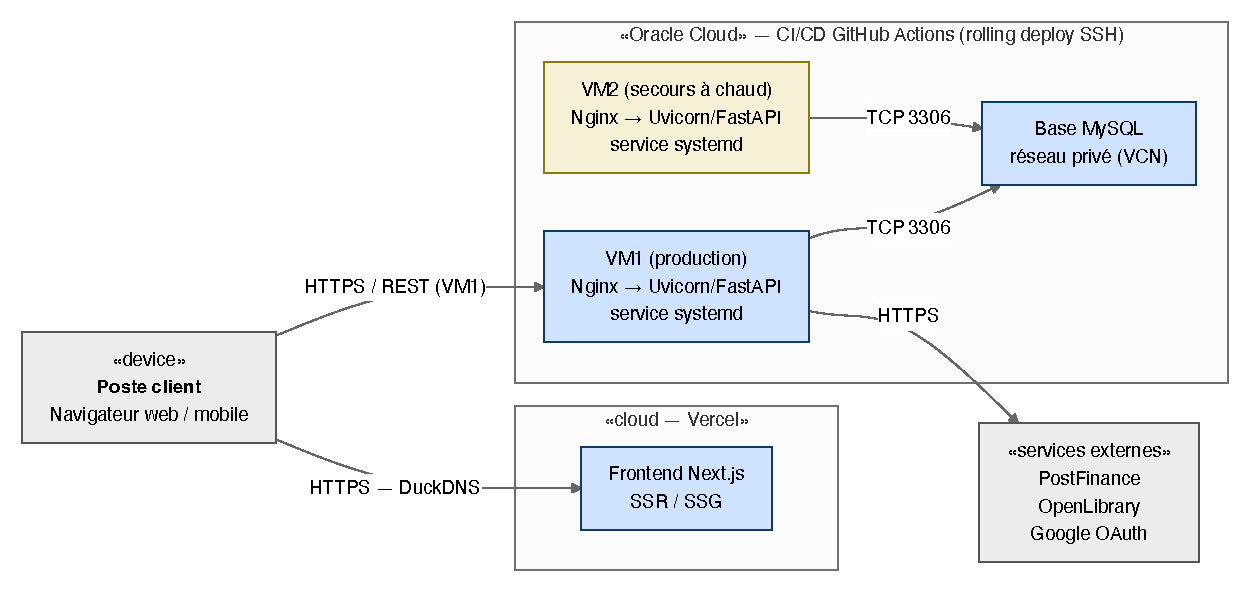
\includegraphics[width=\linewidth,height=0.82\textheight,keepaspectratio]{diagrams/deploiement.pdf}
  \end{center}
\end{frame}

\section{Conclusion \& perspectives}

\begin{frame}{Conclusion --- Bilan et perspectives}
  \begin{columns}[T]
    \column{0.48\textwidth}
    \begin{exampleblock}{Ce que je retiens techniquement}
      \begin{itemize}\small
        \item Les \textbf{4 critères MVP} sont tenus et mesurés
        \item Ce qui m'a le plus appris : la \textbf{concurrence} (verrou stock) et le \textbf{SSRF}
        \item Un outil qui échoue bruyamment vaut mieux qu'un outil permissif
      \end{itemize}
    \end{exampleblock}
    \vspace{4pt}
    \begin{alertblock}{Limites identifiées --- sans complaisance}
      \begin{itemize}\small
        \item Rate limiting \textbf{en mémoire} : ne tient pas sur plusieurs VMs
        \item Aucun test de charge : les perfs sont \textbf{supposées}, pas prouvées
        \item Interface mobile à affiner (responsive)
      \end{itemize}
    \end{alertblock}
    \column{0.48\textwidth}
    \begin{block}{Perspectives d\textquotesingle{}évolution}
      \begin{itemize}\small
        \item \textbf{Phase 2} : messagerie acheteur-vendeur, système d'avis et de notation
        \item \textbf{Phase 3} : estimation de prix IA, étiquettes PostPac, recommandations personnalisées
        \item \textbf{Évolutions tech} : Redis (cache catalogue), CDN images, tests de charge (Locust/k6)
      \end{itemize}
    \end{block}
    \vspace{4pt}
    \begin{exampleblock}{\small Et notre livre, dans tout ça ?}
      \begin{itemize}\small
        \item \textit{Divergente T.2} : scanné, catalogué, acheté, payé, livré
        \item Le même parcours pour chaque livre réel déposé chez Caritas
      \end{itemize}
    \end{exampleblock}
  \end{columns}
\end{frame}

\begin{frame}[plain]
  \begin{tikzpicture}[remember picture,overlay]
    \fill[myblue] (current page.north west) rectangle (current page.south east);
    \fill[mybluelight!40,opacity=0.4]
      (current page.south west) rectangle ++(\paperwidth,0.20\paperheight);
    \fill[white,opacity=0.03] (current page.center) ++(2,1) circle (4.5);
  \end{tikzpicture}
  \vspace{0.8cm}
  \begin{center}
    {\color{white}\fontsize{28}{34}\selectfont\bfseries Merci de votre attention}\\[18pt]
    \begin{tikzpicture}
      \draw[white!50,line width=0.8pt] (0,0) -- (8,0);
    \end{tikzpicture}\\[14pt]
    {\color{white!80}\Large Questions ?}\\[24pt]
    {\color{white}\textbf{Alexandre REY}}\\[5pt]
    {\color{white!70}\small alexandre.rey@qiminfo.ch}\\[8pt]
    {\color{white!70}\small caribooks.vercel.app}\\[4pt]
    {\color{white!70}\small github.com/Visualstudiocodetest/caribooks}
  \end{center}
\end{frame}

\end{document}
